\section{Zielsetzung}
\label{sec:Zielsetzung}
Diodenaser sind von zentraler Bedeutung in der Physik, da mit ihrem starken Output von kohärenten
Licht innerhalb eines schmalen Frequenzsprektrums sehr gut atomare Strukturen bzw. Quantensysteme
untersucht werden können. Außerdem können die Laser auf eine bestimmte Wellenlänge eingestellt werden, 
wodurch sie sich optimal auf das zu untersuchende System anpassen lassen.
In diesem Versuch soll die Funktionsweise eines Diodenlasers näher untersucht werden, indem die
Fluoreszenz von Rubidium nachgewiesen wird. Dafür müssen die verschiedenen Laserparamter so justiert werden,
dass die für Rubidium benötigte Wellenlänge erzeugt wird.

\section{Theorie}
\label{sec:Theorie}

Bevor der Aufbau eines Diodenlaser erläutert wird, folgen zuerst die physikalischen Grundlagen von Photonenemmission
sowie Halbleitern und Dioden, da diese essentiell für das Verständniss der Funktionsweise eines Diodenlasers sind.

\subsection{Absorption und Emmission in Zustandssystemen}
\label{sec:sub1}

In quantenmechanischen Systemen liegen diskrete Energieniveaus vor, das einfachste Beispiel hierfür ist ein Zweizustandssystem
mit einer Grundzustandsenergie $E_1$ und einem angeregten Zustand mit der Energie $E_2$. Um in einen
angeregten Zustand zu wechseln, kann ein Teilchen ein Photon absorbieren, falls die Energie des Photons genau der
Energiedifferenz der Niveaus entspricht:
\begin{equation}
    \notag
    E_{\text{ph}} = E_2 - E_1 = h \omega
\end{equation}
Umgekehrt muss ein Photon emmitiert werden, wenn das Teilchen wieder auf den Grundzustand wechselt.
Die Emmission des Photons kann zufällig erfolgen (spontane Emmission), oder durch ein anderes Photon
ausgelöst werden (stimulierte Emmission). Bei der stimulierten Emmission wird zusätzlich zu dem Photon,
dass die Emmission ausgelöst hat, ein zweites Photon erzeugt. Dieses Photon ist hinsichtlich aller seiner
Eigenschaften wie Frequenz, Polarisation und Phase identisch zum ersten Photon. Somit ist leicht
ersichtlich, warum dieser Vorgang in Lasern ausgenutzt wird. Findet er oft genug statt, so wird eine
ganz spezifische Wellenlänge an Licht starkt verstärkt, die dann zum Experimentieren genutzt werden kann.

Damit die stimulierte Emmission im Vergleich zur spontanen Emmission überwiegen kann, muss der energetisch
höhere Zustand häufiger besetzt sein als der niedrige, dies wird auch als Besetzungsinversion bezeichnet.
In dem zuvor beschriebenen Zweizustandssystem lässt sich dies nicht realisieren. Da die Übergangwahrscheinlichkeit
von $E_1$ zu $E_2$ genau so groß ist wie von $E_2$ zu $E_1$, kann höchstens
eine Gleichbesetzung erreicht werden.

Sobald ein oder mehrere weitere Zustände hinzugefügt werden, kann dieser Effekt jedoch auftreten.
In \autoref{fig:Besetzungsinversion} ist der simpelste Fall, also ein Dreizustandssystem, abgebildet.
\begin{figure}[H]
    \centering
    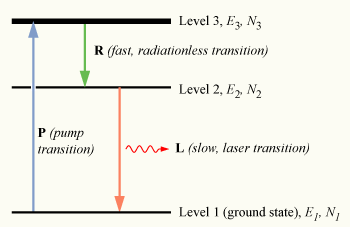
\includegraphics[height=6cm]{content/pics/besetzungsinversion.png}
    \caption{Skizze eines Dreizustandssystems und den möglichen Übergängen. \cite{Besetzungsinversion}}
    \label{fig:Besetzungsinversion}
\end{figure}
Es existiert ein drittes Energieniveau $E_3$, in dass die Teilchen durch die eingehenden Photonen gepumpt werden.
Dannach fallen sie sehr schnell ohne Emmission eines Photons in den mittleren Zustand $E_2$. Von dort aus kann
die zuvor beschriebene, langsamere stimulierte Emmission stattfinden. Alle Teilchen die im Grundzustand landen,
werden durch die anderen Photonen direkt wieder in den höchsten Zustand versetzt. Somit verweilen die meisten
Teilchen im mittleren Zustand $E_2$ und die zuvor beschriebene Besetzungsinversion wurde erreicht.

\subsection{Dioden}
Die Diode ist das zentrale Element, dass die Umwandlung der elektrischen Energie, die dem Laser zugeführt wird, in
kohärentes Licht ermöglicht.
Dafür werden die Eigenschaften von p- und n-dotierten Halbleitern ausgenutzt, beziehungsweise die einer Kombination von beiden.
Ein dotierter Halbleiter ist ein Kristall, in den Fremdatome eingebracht wurden. Bei der p-dotierung handelt es sich um
Fremdatome mit einem Hüllenelektron weniger als die ursprünglichen Atome. Das fehlende Elektron wird als "Loch"\, betrachtet
und verhält sich bereits mit geringer thermischer Anregung (Raumtemperatur) wie in positives Teilchen, dass sich frei bewegen kann.
Ein n-dotierter Halbleiter verfügt über Fremdatome mit einem zusätzlichen Hüllenelektron, welches sich nach Anregung dann ebenfalls frei
bewegen kann.
Eine Diode konstruiert man nun, indem man einen p- und n-dotierten Halbleiter zusammenfügt, sodass ein Übergang zwischen den
beiden Zonen entsteht. An dem Übergang können Elektronen und Löcher ausgetauscht werden, sodass eine Zone negativer Ladung
im p-dotierten Teil und eine Zone positiver Ladung im n-dotierten Teil entsteht.
In dieser Zone können sich keine freien Ladungsträger mehr aufhalten, daher wird sie auch als Sperrschicht bezeichnet.
Die Situation ist in \autoref{fig:pn} skizziert.
\begin{figure}[H]
    \centering
    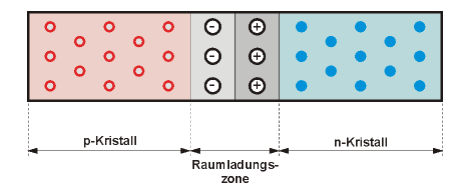
\includegraphics[height=4cm]{content/pics/pn_uebergang.png}
    \caption{Schematische Darstellung eines pn-Übergangs. \cite{pn_uebergang}}
    \label{fig:pn}
\end{figure}
Nun wird eine Spannung angelegt, dabei ist die Polung entscheidend, da der pn-Übergang nur in einer Richtung stromdurchlässig ist.
Sobald ein Strom durch die Diode fließt, beginnen die Elektron-Loch Paare zu rekombinieren und senden dabei Photonen aus, der
Vorgang ist in \autoref{fig:pn_strom} dargestellt.
\begin{figure}[H]
    \centering
    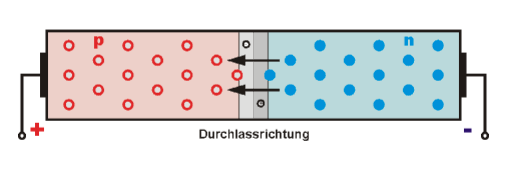
\includegraphics[height=3.5cm]{content/pics/pn_strom.png}
    \caption{Schematische Darstellung eines pn-Übergangs bei angelegter Spannung. \cite{pn_uebergang}}
    \label{fig:pn_strom}
\end{figure}
Energetisch liegt hier ein Vierniveausystem vor, also analog zu dem in \autoref{sec:sub1} beschriebenen System mit einem
zusätzlichen Energieniveau knapp über der Grundzustandsenergie. Bei ausreichend großen Stromstärken werden genug Photonen emmitiert, um eine Besetzungsinversion
zu erreichen. Dann findet in der Diode stimulierte Emmission statt und es entsteht kohärentes Licht mit hoher Intensität, da die
emmitierten Photonen direkt weitere, identische Photonen erzeugen können.

\subsection{Aufbau eines Diodenlasers und Justierung}

\begin{figure}[H]
    \centering
    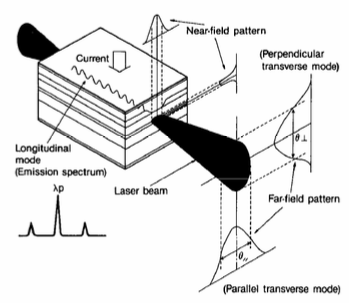
\includegraphics[height=8cm]{content/pics/laser.png}
    \caption{Laserskizze. \cite{V60}}
    \label{fig:laser}
\end{figure}

\begin{figure}[H]
    \centering
    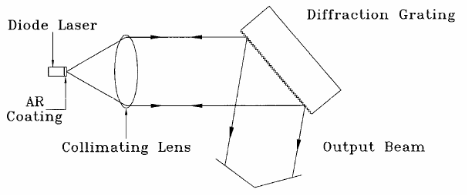
\includegraphics[height=5cm]{content/pics/graiting.png}
    \caption{graiting. \cite{V60}}
    \label{fig:graiting}
\end{figure}

\begin{figure}[H]
    \centering
    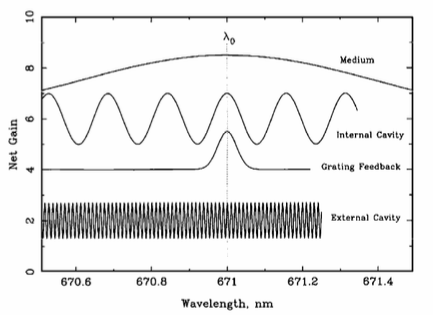
\includegraphics[height=5cm]{content/pics/gain.png}
    \caption{gain. \cite{V60}}
    \label{fig:grain}
\end{figure}

\subsection{Absorptionsspektrum von Rubidium}

\begin{figure}[H]
    \centering
    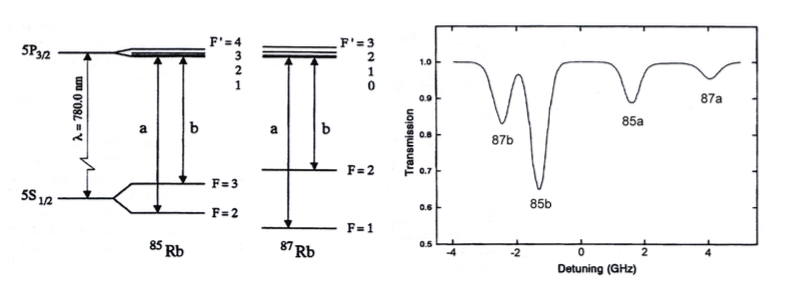
\includegraphics[height=5cm]{content/pics/Rubidium.png}
    \caption{Rubidium. \cite{V60}}
    \label{fig:rubidium}
\end{figure}

